\documentclass[tikz,border=10pt]{standalone}
\usepackage{tikz}
\usetikzlibrary{calc}

\begin{document}
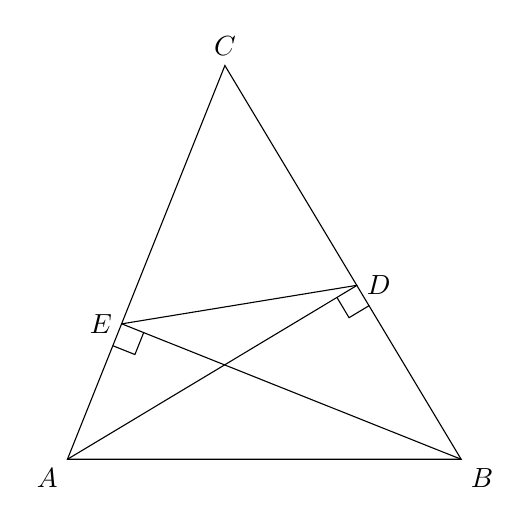
\begin{tikzpicture}
    \coordinate (A) at (0,0);
    \coordinate (B) at (5,0);
    \coordinate (C) at (2,5);
    \coordinate (D) at (3.68, 2.21);
    \coordinate (E) at (0.69, 1.72);

    \draw (A) -- (B) -- (C) -- cycle;
    \draw (A) -- (D);
    \draw (B) -- (E);
    \draw (D) -- (E);

    \draw ($(D)!3mm!(A)$) -- ($(D)!3mm!(A) + ($(D)!3mm!(B)$) - (D)$) -- ($(D)!3mm!(B)$);
    \draw ($(E)!3mm!(B)$) -- ($(E)!3mm!(B) + ($(E)!3mm!(A)$) - (E)$) -- ($(E)!3mm!(A)$);

    \node[below left] at (A) {$A$};
    \node[below right] at (B) {$B$};
    \node[above] at (C) {$C$};
    \node[right] at (D) {$D$};
    \node[left] at (E) {$E$};
\end{tikzpicture}
\end{document}
